\documentclass[a4paper,10pt]{scrartcl}
\usepackage[utf8]{inputenc}
\usepackage[spanish]{babel} 
\usepackage[hidelinks]{hyperref}
\usepackage{color}
\usepackage[table,xcdraw]{xcolor}
\usepackage{array}
\newcolumntype{M}[1]{>{\centering\arraybackslash}m{#1}}

\usepackage{graphicx}
\usepackage{float}
\graphicspath{ {images/} }


\title{Alcance del proyecto}
\subtitle{Grupo 1.2.2 - Redmine}
\author{
		Manuel Francisco López Ruiz\\
		Julio Márquez Castro\\
		Álvaro Martín Gordillo\\
		  }

\begin{document}

\clearpage\maketitle
\thispagestyle{empty}
\newpage
\begin{center}
	\begin{table}
		\centering
		\begin{tabular}{| c | M{2cm} | M{2cm} | M{2cm} | c | M{3cm} |}
			\hline
			\multicolumn{6}{|c|}{\textbf{Control de versiones}} \\ \hline
			\textbf{Ver.} & \textbf{Hecha por} & \textbf{Revisada por} & \textbf{Aprobada por} & \textbf{Fecha} & \textbf{Motivo} \\ \hline
			0.1 & Manuel Francisco López Ruiz y Julio Márquez Castro  & Álvaro Martín Gordillo & -- & 25/11/2016 & Creación del Alcance \\ \hline

			1.0 & Manuel Francisco López Ruiz y Julio Márquez Castro  & Álvaro Martín Gordillo & -- & 07/12/2016 & Revisión final \\ \hline
		\end{tabular}
	\end{table}
\end{center}

\newpage

\tableofcontents

\newpage



\section{Objetivos del proyecto}

Obtener un alto nivel de conocimientos sobre la herramienta Redmine con el fin de ser capaces de transmitir los conocimientos aprendidos.

\section{Descripción del producto o servicio}

El servicio es un curso introductorio a Redmine donde se debe explicar que es, como se usa, errores comunes y ventajas e inconvenientes frente a otros servicios. Tras la explicación se realizará una práctica con el objetivo de que los asistentes puedan practicar los conceptos aprendidos y preguntar dudas.

\section{Requisitos del proyecto/producto}

\begin{itemize}
	\item Software Redmine
	\item Acceso a internet
	\item Servidor para Redmine
	\item Pc cliente
\end{itemize}

\section{Límites/restricciones del proyecto}

\begin{itemize}
	\item Limite de tiempo del vídeo tutorial
\end{itemize}

\section{Entregables}

El proyecto constará de un único entregable cuya fecha será el 7 de diciembre del año 2016 el cual contendrá:
	\begin{itemize}
		\item Un plan de gestión del trabajo el cual deberá incluir al menos:
		
		\begin{itemize}
			\item Acta de constitución.
			\item Definición del alcance.
			\item Planificación inicial y final.
			\item Lecciones aprendidas.
		\end{itemize}
		
		\item Un tutorial/vídeo destacando los aspectos más importantes del trabajo propuesto.
		
		\item Un enunciado de un ejemplo práctico con la resolución del mismo.
		
		\item La presentación de la exposición de la práctica que se realizará públicamente. Para ello, y a indicaciones del profesorado se podrá utilizar el tutorial/vídeo.		
	\end{itemize}

Así mismo se realizará una presentación del trabajo el 9 de diciembre del año 2016 con una duración máxima de 35 minutos constando de:
\begin{itemize}
	\item Descripción del trabajo realizado y lecciones aprendidas.
	
	\item Reproducción del vídeo de presentación global de la herramienta.
	
	\item Tutorial dirigido. El mismo debe constar de un ejercicio práctico para los asistentes a resolver en el tiempo disponible y aportar la solución del mismo.

	\item Preguntas.


\end{itemize}

\section{Criterios de aceptación}
El profesorado de la asignatura evaluará la calidad de los contenidos de la memoria y el tutorial/vídeo; la claridad de la exposición en la presentación y la adecuación del enunciado presentado.

\section{Exclusiones}
Será excluido en caso de que no se presente lo requerido en los entregables o que la calidad del contenido sea muy pobre e incompleta.


\section{Asunciones}

	\begin{enumerate}
		\item Podremos realizar toda la documentación necesaria con \LaTeX.
		
		\item Podremos aprender y trabajar con GIT\footnote{\url{https://git-scm.com/}}/GitHub\footnote{\url{https://github.com/}} sin ningún problema.
		
		\item Dispondremos de acceso a internet para poder usar las herramientas necesarias para el desarrollo.

		\item No habrá ninguna evaluación más a las descritas en este documento.
		
		\item Colaboración permanente por parte de los integrantes del grupo para la realización de la práctica.
		
		\item Cumplir con todos los objetivos establecidos por el grupo de trabajo.
		
		\item Contacto con los profesores de la asignatura para una revisión del proyecto
	\end{enumerate}


\section{Riesgos iniciales}

Los riesgos iniciales encontrados son los siguientes:
\begin{enumerate}
	\item Desconocimiento por parte de parte del equipo de las herramientas usadas para el desarrollo de la documentación \LaTeX y GIT\footnote{\url{https://git-scm.com/}}/GitHub\footnote{\url{https://github.com/}}.
	
	\item Desconocimiento por todo el equipo de como realizar un vídeo tutorial.
	
	\item Desconocimiento parcial del uso para el que se debe realizar el tutorial (Redmine\footnote{\url{http://www.redmine.org/}}) puesto que ProjETSII\footnote{\url{https://projetsii.informatica.us.es/}} es una modificación del mismo pero no es igual.
	
	\item Realizar una mala planificación que dificulte o llegue a cancelar el proyecto.
	
	\item Falta de experiencia con este tipo de proyectos que ocasionen dudas en la realización de documentación 
\end{enumerate}


\section{Fechas importantes}
Las fechas importantes serán las siguientes:

	\begin{itemize}
		\item 28 de octubre del año 2016: Primera sesión de seguimiento del trabajo.
		
		\item 2 de diciembre del año 2016: Segunda sesión de seguimiento del trabajo.
		
		\item 7 de diciembre del año 2016: Entrega documentación y tutorial/vídeo.
		
		\item 9 de diciembre del año 2016: Presentación.
	\end{itemize}

\section{EDT}

	\begin{center}
		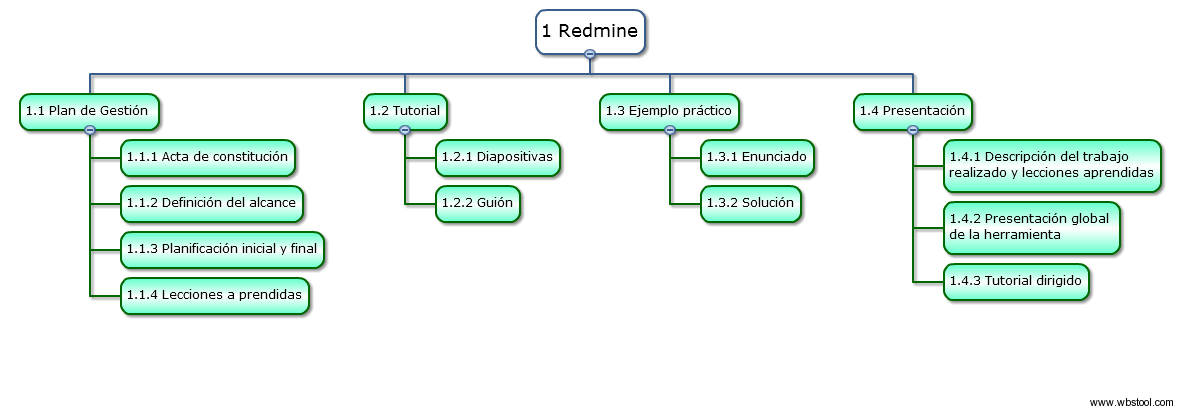
\includegraphics[width=\linewidth]{EDT}
	\end{center}

\section{Diccionario EDT}

\begin{table}[H]
	\centering
	\begin{tabular}{|c|M{3cm}|M{8cm}|}
		\hline
		\textbf{Código} & \textbf{Nombre}          & \textbf{Descripción}                                    \\ \hline
		1.1    & Plan de Gestión & Documentación de la planificación del proyecto \\ \hline
		1.1.1  & Acta de constitución & Documento que autoriza el inicio del proyecto, donde se recogen requisitos y expectativas, con información de alto nivel.   \\ \hline
		1.1.2  & Definición del alcance & Documento que se elabora a partir de los entregables principales del proyecto, donde incluimos objetivos, requisitos, riesgos, fechas. \\ \hline
		1.1.3  & Planificación inicial y final & Documento donde incluimos las tareas que hay que realizar a lo largo del proyecto, con sus tiempos estimados en la planificación inicial y los tiempos reales al final del proyecto. Esto nos permite valorar si se hicieron buenas estimaciones al comienzo del proyecto.  \\ \hline
		1.1.4  & Lecciones aprendidas & Documentación sobre los conceptos aprendidos tanto del software tutorizado como de las técnicas y herramientas usadas para la elaboración del tutorial y la documentación. \\ \hline
		1.2    & Tutorial & Vídeo-tutorial sobre el software Redmine. \\ \hline
		1.2.1  & Vídeo & Vídeo de introducción a Redmine, incluyendo los aspectos básicos sobre el software, ampliando los conceptos en el tutorial dirigido. \\ \hline
		1.2.2  & Guión & Pequeña guía usada para la creación del vídeo-tutorial. \\ \hline
		1.3    & Ejemplo Práctico & Ejercicio de ejemplo para presentar el software. \\ \hline
		1.3.1  & Enunciado & Ejercicio planteado por el grupo de trabajo para tutorizar al resto de los compañeros. \\ \hline
		1.3.2  & Solución & Solución planteada al ejercicio propuesto. \\ \hline
		1.4    & Presentación & Exposición del trabajo en clase con el resto de los compañeros. \\ \hline
		1.4.1  & Descripción del trabajo realizado y lecciones aprendidas & Diapositivas sobre el equipo de trabajo, trabajo realizado y las lecciones aprendidas para presentar al resto de los compañeros. \\ \hline
		1.4.2  & Presentación global de la herramienta & Presentación del software Redmine. \\ \hline
		1.4.3  & Tutorial dirigido & Realización del ejercicio propuesto en clase con el resto de los compañeros. \\ \hline
	\end{tabular}
	\caption{Diccionario EDT}
	\label{table:edt}

\end{table}

\bibliography{sample}

\end{document}
